\documentclass[8pt,aspectratio=169]{beamer}
\usetheme[block=fill]{ru}           % Use ru theme

\usepackage{common}
\newtheorem{theorem}{Theorem}[section]
\newtheorem{lemma}[theorem]{Lemma}
\newtheorem{proposition}[theorem]{Proposition}
\newtheorem{corollary}[theorem]{Corollary}

\newcommand\invisiblesection[1]{%
  \refstepcounter{section}
\sectionmark{#1}}

\newenvironment{proof}[1][Proof]{\begin{trivlist}
\item[\hskip \labelsep {\bfseries #1}]}{\end{trivlist}}
  \newenvironment{definition}[1][Definition]{\begin{trivlist}
\item[\hskip \labelsep {\bfseries #1}]}{\end{trivlist}}
  \newenvironment{example}[1][Example]{\begin{trivlist}
\item[\hskip \labelsep {\bfseries #1}]}{\end{trivlist}}
  \newenvironment{remark}[1][Remark]{\begin{trivlist}
\item[\hskip \labelsep {\bfseries #1}]}{\end{trivlist}}

  \newcommand{\qed}{\nobreak \ifvmode \relax \else
    \ifdim\lastskip<1.5em \hskip-\lastskip
    \hskip1.5em plus0em minus0.5em \fi \nobreak
  \vrule height0.75em width0.5em depth0.25em\fi}


% \DeclareMathOperator*{\argmin}{arg\,min}
% \DeclareMathOperator*{\Vol}{Vol}
% \DeclareMathOperator*{\Supp}{Supp}
% \newcommand{\cR}{\ensuremath{\mathcal R}}
% \newcommand{\cS}{\ensuremath{\mathcal S}}
%
% \newcommand{\CVPDf}{\ensuremath{\algo{CVP}_{\tilde{D}_4}}}
% \newcommand{\CVPDfZf}{\ensuremath{\algo{CVP}_{D_4/\ZZ^4}}}
% \newcommand{\LDEncode}{\algo{Encode}}
% \newcommand{\LDDecode}{\algo{Decode}}



\usepackage{soul}\let\strikethrough\st\let\st\undefined

% \newcommand{\T}{L}

\newcommand{\Z}{\ensuremath{\mathbb{Z}}}
\newcommand{\K}{\ensuremath{\mathbb{K}}}
\newcommand{\ZZ}{\ensuremath{\mathbb{Z}}}
\newcommand{\corr}{\,\hat{=}\,}
\newcommand{\B}{\ensuremath{\mathbb{B}}}
\newcommand{\E}{\ensuremath{\mathbb{E}}}
\newcommand{\Oinf}{\ensuremath{\mathcal{O}}}
\newcommand{\F}[1]{\ensuremath{\mathbb{F}_{#1}}}

% \newcommand{\RR}{\ensuremath{\mathbb{R}}}
\newcommand{\N}{\ensuremath{\mathbb{N}}}

\newcommand{\mbf}{\ensuremath{\mathbf}}
% \newcommand{\rando}{\ensuremath{\xleftarrow{\$}}}
% \newcommand{\la}{\ensuremath{\leftarrow}}

% \newcommand{\MD}{\ensuremath{\mathcal{D}}\xspace}
% \newcommand{\MS}{\ensuremath{\mathcal{D}}\xspace}
% \newcommand{\MA}{\ensuremath{\mathcal{A}}\xspace}
% \newcommand{\MB}{\ensuremath{\mathcal{B}}\xspace}
% \newcommand{\MP}{\ensuremath{\mathcal{P}}\xspace}
% \newcommand{\tA}{\ensuremath{t_{\mathcal{A}}}}
% \newcommand{\eA}{\ensuremath{\varepsilon_{\mathcal{A}}}}
% \newcommand{\tS}{\ensuremath{t_{\mathcal{D}}}}
% \newcommand{\eS}{\ensuremath{\varepsilon_{\mathcal{D}}}}

% \newcommand{\vX}{\mathcal X}
% \newcommand{\vY}{\mathcal Y}


% \newcommand{\MR}{\ensuremath{\mathcal{R}}\xspace}
% \newcommand{\tR}{\ensuremath{t_{\mathcal{R}}}}
% \newcommand{\eR}{\ensuremath{\varepsilon_{\mathcal{R}}}}
%
% \newcommand{\tD}{\ensuremath{t_{\mathcal{D}}}}
% \newcommand{\eD}{\ensuremath{\varepsilon_{\mathcal{D}}}}
% \newcommand{\sis}{\textsf{SIS}\xspace}
% \newcommand{\isis}{\textsf{ISIS}\xspace}
% \newcommand{\lwe}{\textsf{LWE}\xspace}
% \newcommand{\dlwe}{\textsf{LWE}\xspace}
% \newcommand{\rdlwe}{\textsf{R-LWE}\xspace}
%
% \newcommand{\ee}{\ensuremath{\varepsilon}}
%
% \newcommand{\sS}{\ensuremath{\sigma}}
% \newcommand{\sE}{\ensuremath{\sigma}}
% \newcommand{\DS}{\ensuremath{D_{\sS}}}
% \newcommand{\DE}{\ensuremath{D_{\sE}}}
% %\newcommand{\Dy}{\ensuremath{D_y}}
% \newcommand{\Dy}{\ensuremath{[-B, B]}}
% \newcommand{\Dysc}{\ensuremath{D_{y,\mat{Sc}}}}
% \newcommand{\Dz}{\ensuremath{D_z}}
% \newcommand{\bit}{\ensuremath{\{0,1\}}}
% \newcommand{\eqdef}{\stackrel{\mathrm{def}}=}
% \newcommand{\rand}{\getsr}

% \newcommand{\rounddq}[1]{\ensuremath{\lfloor #1 \rceil_{d,q}}}
% \newcommand{\roundd}[1]{\ensuremath{\lfloor #1 \rceil_d}}
% \newcommand{\norm}[1]{\ensuremath{||#1||}}

% \newcommand{\KeyGen}{\keygen}
% \newcommand{\Sign}{\sign}
% \newcommand{\Verify}{\verify}
% \newcommand{\keygen}{\ensuremath{\mathsf{KeyGen}}}
% \newcommand{\sign}{\ensuremath{\mathsf{Sign}}}
% \newcommand{\verify}{\ensuremath{\mathsf{Verify}}}
% \newcommand{\start}{\underline{\ensuremath{\mathsf{Start}}}\xspace}
% \newcommand{\randO}{\ensuremath{\underline{\mathsf{Rand}}^{O_c}}\xspace}
% \newcommand{\signO}{\ensuremath{\underline{\mathsf{Sign}}^{O_c}}\xspace}
% \newcommand{\finishO}{\ensuremath{\underline{\mathsf{Finish}}^{O_c}}}
% \newcommand{\instance}{\underline{\ensuremath{\mathsf{Instance}}}}
% \newcommand{\Sample}{\ensuremath{\mathsf{Sample}}}

% \newcommand{\keygenQ}{\ensuremath{\mathsf{KeyGen}}}
% \newcommand{\signQ}{\ensuremath{\mathsf{Sign}}}
% \newcommand{\verifyQ}{\ensuremath{\mathsf{Verify}}}
% \newcommand{\CHgen}{\ensuremath{\mathsf{ChGen}}}

% \newcommand{\inputtext}{\textsf{INPUT:}\;}
% \newcommand{\outputtext}{\textsf{OUTPUT:}\;}
% \newcommand{\iftext}{\mathbf{if\;}}
% \newcommand{\elsetext}{\mathbf{else\;}}
% \newcommand{\then}{\mathbf{then\;}}
% \newcommand{\return}{\mathbf{return\;}}

% \newcommand{\mat}[1]{\mathbf{#1}}
% \renewcommand{\vec}[1]{\mathbf{#1}}
% \newcommand{\modq}{\ensuremath{\; (\bmod \; q)}}
%\newcommand{\modq}{\ensuremath{\; (q)}}
% \newcommand{\ip}[2]{\ensuremath{\langle {#1},{#2}\rangle}}

% \newcommand{\adv}{\ensuremath{\mathcal{A}}}
% \newcommand{\secpar}{\ensuremath{\lambda}}

% \newcommand{\sk}{\ensuremath{\mathsf{sk}}\xspace}
% \newcommand{\pk}{\ensuremath{\mathsf{vk}}\xspace}
% \newcommand{\sst}{\ensuremath{\mathsf{st}}\xspace}

% \newcommand{\CH}{\ensuremath{\mathcal{CH}}}
% \newcommand{\ch}{\ensuremath{\mathsf{CH}}}
% \newcommand{\Mek}{\ensuremath{\mathsf{M_{ek}}}}
% \newcommand{\Yek}{\ensuremath{\mathsf{Y_{ek}}}}
% \newcommand{\Rek}{\ensuremath{\mathsf{R_{ek}}}}
% \newcommand{\ek}{\ensuremath{\mathsf{ek}}}
% \newcommand{\td}{\ensuremath{\mathsf{td}}}
% \newcommand{\Gen}{\ensuremath{\mathsf{Gen}}}

% \newcommand{\negl}{\ensuremath{\mathsf{negl}}}


% \newcommand{\R}{\mathcal{R}}
% \newcommand{\Rp}{\mathcal{R}_p}
% \newcommand{\Rq}{\mathcal{R}_q}
% \newcommand{\Rqk}[1]{\mathcal{R}_{q,#1}}

% \def\getsr{\stackrel{{\scriptscriptstyle \$}}{\leftarrow}}
% \def\gets{{\leftarrow}}


% \newcommand{\Uniform}{\mathcal{U}}
% \newcommand{\UniRk}[1]{\Rqk{#1}}
% \newcommand{\UniRq}{\Rq}


\newcommand{\zeropo}{{\bf 0}}
\newcommand{\Apo}{{\bf A\xspace}}
\newcommand{\Bpo}{{\bf B\xspace}}
\newcommand{\Ipo}{{\bf I\xspace}}
\newcommand{\apo}{{\bf a\xspace}}
\newcommand{\bpo}{{\bf b\xspace}}
\newcommand{\cpo}{{\bf c\xspace}}
\newcommand{\Cpo}{{\bf C\xspace}}
\newcommand{\dpo}{{\bf d\xspace}}
\newcommand{\epo}{{\bf e\xspace}}
\newcommand{\ppo}{{\bf p\xspace}}
\newcommand{\fpo}{{\bf f\xspace}}
\newcommand{\gpo}{{\bf g\xspace}}
\newcommand{\Gpo}{{\bf G\xspace}}
\newcommand{\hpo}{{\bf h\xspace}}
\newcommand{\kpo}{{\bf k\xspace}}
\newcommand{\Kpo}{{\bf K\xspace}}
\newcommand{\lpo}{{\bf l\xspace}}
\newcommand{\Lpo}{{\bf L\xspace}}
\newcommand{\mpo}{{\bf m\xspace}}
\newcommand{\rpo}{{\bf r\xspace}}
\newcommand{\spo}{{\bf s\xspace}}
\newcommand{\tpo}{{\bf t\xspace}}
\newcommand{\upo}{{\bf u\xspace}}
\newcommand{\Upo}{{\bf U\xspace}}
\newcommand{\vpo}{{\bf v\xspace}}
\newcommand{\wpo}{{\bf w\xspace}}
\newcommand{\xpo}{{\bf x\xspace}}
\newcommand{\ypo}{{\bf y\xspace}}
\newcommand{\zpo}{{\bf z\xspace}}
\newcommand{\Zpo}{{\bf Z\xspace}}

\newcommand{\Spo}{{\bf S}}
\newcommand{\Ypo}{{\bf Y}}

% \newcommand{\algo}[1]{\textsf{#1}}

% \newcommand{\PeikertDBL}{\algo{dbl}}
% \newcommand{\PeikertREC}{\algo{rec}}


% \newcommand{\PowMul}{{\text{\sf PowMul}}}
% \newcommand{\PowMulPsi}{{\text{\sf PowMul}_{\psi}}}
\newcommand{\ie}{{\textit{i.e.}}\;}
\newcommand{\eg}{{\textit{e.g.}}\;}
\newcommand{\p}{\ensuremath{2^{255}-19}}
\newcommand{\Zfield}{\ensuremath{\mathbb{Z}_{\p}}}
\newcommand{\Ffield}{\ensuremath{\mathbb{F}_{\p}}}


\mode<presentation>{}


\newcommand{\chapternote}[1]{{%
  \let\thempfn\relax% Remove footnote number printing mechanism
  \footnotetext[0]{#1}% Print footnote text
}}

%% preamble
\title{A Coq proof of the correctness of X25519 in TweetNaCl}
% \subtitle{Coq }
\author[Beno\^{i}t Viguier MSc]{
Peter Schwabe,
\textbf{Beno\^{i}t Viguier},
Timmy Weerwag,
Freek Wiedijk\\
}

\institute[Radboud University Nijmegen]{
  Institute for Computing and Information Sciences -- Digital Security \\
  Radboud University, Nijmegen}

\date[24, Jun. 2021]{
  34$^{th}$ IEEE Computer Security Foundations Symposium\\
  June 24$^{th}$, 2021}


\setbeamertemplate{navigation symbols}{}
\begin{document}


%%%%%%%%%%%%%%%%%%%%%%%%%%%%%%%%%
%
%			SLIDE TITLE
%
%%%%%%%%%%%%%%%%%%%%%%%%%%%%%%%%%
\begin{frame}
	\titlepage
\end{frame}


%%%%%%%%%%%%%%%%%%%%%%%%%%%%%%%%%
%
%     SLIDE CONTENT
%
%%%%%%%%%%%%%%%%%%%%%%%%%%%%%%%%%
% \begin{frame}{Overview}
% \tableofcontents
% \end{frame}


%%%%%%%%%%%%%%%%%%%%%%%%%%%%%%%%%
%
%     SLIDE OVERVIEW
%
%%%%%%%%%%%%%%%%%%%%%%%%%%%%%%%%%19
\begin{frame}{Overview}
	\begin{tikzpicture}[textstyle/.style={black, anchor= south west, align=center, minimum height=0.45cm, text centered, font=\scriptsize}]


  % adapt line thickness and line width, if needed

   \path [thick, dashed] (2.5,1) edge +(0,-6.75);
   \draw (2.5,1) node[anchor=north east] {\sref{sec:Coq-RFC}};
   \draw (2.5,1) node[anchor=north west] {\sref{sec:C-Coq}};
   \path [thick, dashed] (0,-5.75) edge +(8.5,0);
   \draw (8.5,-5.75) node[anchor=north east] {\sref{sec:maths}};

  % SECTION III

  % Definition of RFC
  \begin{scope}[yshift=-3 cm,xshift=0 cm]
   \draw (0,0) -- (0.4, 0.4) -- (1.75,0.4) -- (1.75,0) -- cycle;
   \draw (0,0) -- (1.75,0) -- (1.75,-1) -- (0, -1) -- cycle;
   \draw (0.3,-0.05) node[textstyle] {Definition};
   \draw (0.875,-0.5) node[textstyle, anchor=center] {\texttt{RFC}};
   \draw (1.75,-1) node[textstyle, anchor = south east] {\color{doc@lstfunctions}{.V}};
  \end{scope}

   % SECTION IV

  % C code
  \begin{scope}[yshift=-0.25 cm,xshift=2.75 cm]
    \draw (0,0) -- (0.4, 0.4) -- (1.25,0.4) -- (1.25,0) -- cycle;
    \draw (0,0) -- (1.25,0) -- (1.25,-1.25) -- (0, -1.25) -- cycle;
    \draw (0.3,-0.05) node[textstyle] {code};
    \draw (0.675,-0.5) node[textstyle, anchor=center] {\texttt{Prog}};
    \draw (1.25,-1.25) node[textstyle, anchor = south east] {\color{doc@lstfunctions}{.C}};
  \end{scope}

  % V code
  \begin{scope}[yshift=-0.25 cm,xshift=5 cm]
    \draw (0,0) -- (0.4, 0.4) -- (1.25,0.4) -- (1.25,0) -- cycle;
    \draw (0,0) -- (1.25,0) -- (1.25,-1.25) -- (0, -1.25) -- cycle;
    \draw (0.3,-0.05) node[textstyle] {code};
    \draw (0.675,-0.5) node[textstyle, anchor=center] {\texttt{Prog}};
    \draw (1.25,-1.25) node[textstyle, anchor = south east] {\color{doc@lstfunctions}{.V}};
    % \draw (1.25,0)  node[anchor=south east, inner sep=0pt] {
\includegraphics[width=.0125\textwidth]{img/coq_logo.png}};
  \end{scope}

  \path [thick, dotted, double, ->] (4,-0.75) edge (5, -0.75);

  % VST Spec
  \begin{scope}[yshift=-3 cm,xshift=2.75 cm]
    \draw (0,0) -- (0.4, 0.4) -- (2.75,0.4) -- (2.75,0) -- cycle;
    \draw (0,0) -- (2.75,0) -- (2.75,-2) -- (0, -2) -- cycle;
    \draw (0.3,-0.05) node[textstyle] {Specification};
    \draw (1.375,-1) node[textstyle, anchor=center, align=left] {
      {\color{doc@lstnumbers}\textbf{Pre}}:\\
      ~~\texttt{s}$[\!\!\{$\texttt{n}$\}\!\!]\leftarrow n \in \N$,\\
      % ~~$n \in$ \TNaCles{u8[32]},\\
      ~~\texttt{s}$[\!\!\{$\texttt{p}$\}\!\!]\leftarrow P \in E(\F{p^2})$\\
      % ~~$P \in$ \TNaCles{u8[32]}\\
      {\color{doc@lstdirective}\textbf{Post}}:\\
      ~~\texttt{s}$[\!\!\{$\texttt{q}$\}\!\!]\leftarrow$~\texttt{RFC}$(n,P)$};
      \draw (2.75,-2) node[textstyle, anchor = south east] {\color{doc@lstfunctions}{.V}};
  \end{scope}

  % VST Theorem
  \begin{scope}[yshift=-3 cm,xshift=6 cm]
    \draw (0,0) -- (0.4, 0.4) -- (2.5,0.4) -- (2.5,0) -- cycle;
    \draw (0,0) -- (2.5,0) -- (2.5,-1.25) -- (0, -1.25) -- cycle;
    \draw (0.3,-0.05) node[textstyle] {Proof};
    \draw (1.25,-0.5) node[textstyle, anchor=center] {\{{\color{doc@lstnumbers}\textbf{Pre}}\} \texttt{Prog} \{{\color{doc@lstdirective}\textbf{Post}}\}};
    \draw (2.5,0) node[textstyle, anchor = south east] {\color{doc@lstfunctions}{\checkmark}};
    \draw (2.5,-1.25) node[textstyle, anchor = south east] {\color{doc@lstfunctions}{.V}};
  \end{scope}

  \path [thick, double] (5.625,-1.5) edge [out=-90, in=90] (5.625, -2.5);
  \path [thick, double, ->] (5.625, -2.5) edge [out=-90, in=180] (6, -3.5);
  \path [thick, double, ->] (5.5,-3.75) edge [out=0, in=180] (6, -3.75);



  % SECTION V

  % Spec of Curve nP
  \begin{scope}[yshift=-7.5 cm,xshift=0 cm]
    \draw (0,0) -- (0.4, 0.4) -- (1.75,0.4) -- (1.75,0) -- cycle;
    \draw (0,0) -- (1.75,0) -- (1.75,-1) -- (0, -1) -- cycle;
    \draw (0.3,-0.05) node[textstyle] {Definition};
    \draw (0.875,-0.5) node[textstyle, anchor=center] {$n \cdot P$};
    \draw (1.75,-1) node[textstyle, anchor = south east] {\color{doc@lstfunctions}{.V}};
  \end{scope}

  % Correctness Theorem
  \begin{scope}[yshift=-7 cm,xshift=6 cm]
    \draw (0,0) -- (0.4, 0.4) -- (2.5,0.4) -- (2.5,0) -- cycle;
    \draw (0,0) -- (2.5,0) -- (2.5,-1.5) -- (0, -1.5) -- cycle;
    \draw (0.3,-0.05) node[textstyle] {Proof};
    \draw (1.25,-0.75) node[textstyle, anchor=center] {{\color{doc@lstnumbers}\textbf{Pre}} $\implies$\\$\text{\texttt{RFC}}(n,P) = n \cdot P$};
    \draw (2.5,0) node[textstyle, anchor = south east] {\color{doc@lstfunctions}{\checkmark}};
    \draw (2.5,-1.5) node[textstyle, anchor = south east] {\color{doc@lstfunctions}{.V}};
  \end{scope}

  \path [thick, double, ->] (1.75,-3.5) edge  [out=0, in=-180] (2.75, -3.5);
  \path [thick, double] (1.75,-3.5) edge [out=0, in=90] (2.25, -4);
  \path [thick, double] (2.25, -4) edge [out=-90, in=90] (2.25, -7);
  \path [thick, double] (2.25, -7) edge [out=-90, in=-180] (3, -7.75);
  \path [thick, double, ->] (3, -7.75) edge [out=0, in=-180] (6, -7.75);
  \path [thick, double, ->] (1.75,-8) edge [out=0, in=-180] (6, -8);


\end{tikzpicture}

\end{frame}


\section{Prelude}

%%%%%%%%%%%%%%%%%%%%%%%%%%%%%%%%%
%
%     SLIDE 2 bis
%
%%%%%%%%%%%%%%%%%%%%%%%%%%%%%%%%%
\begin{frame}[fragile]{Diffie-Hellman with Elliptic Curves}

	\begin{center}
		\begin{tikzpicture}
			\node[draw=none,align=center] (public) at (0,1) {Public parameter: point $P$, curve $E$ over $\K$};

			% Alice
			\node[draw] (Alice) at (-2,0) {Alice};
			\draw[->,thick,>=stealth] (Alice) -- ++(0, -4.5);

			% Calculations of Alice
			\node[draw=none,anchor=east] (asecret) at ($(Alice) + (0,-1)$) {$random\ a \in \N$};
			\node[draw=none,anchor=east] (Apublic) at ($(Alice) + (0,-2)$) {$A = a \cdot P$};
			\node[draw=none,anchor=east] (akey) at ($(Alice) + (0,-4)$) {$S = a \cdot B = (a*b) \cdot  P$};

			% Bob
			\node[draw] (Bob) at (2,0) {Bob};
			\draw[->,thick,>=stealth] (Bob) -- ++(0, -4.5);

			% Calculations of Bob
			\node[draw=none,fill=none,anchor=west] (bsecret) at ($(Bob) + (0,-1)$) {$random\ b \in \N$};
			\node[draw=none,fill=none,anchor=west] (Bpublic) at ($(Bob) + (0,-2)$) {$B = b \cdot P$};
			\node[draw=none,fill=none,anchor=west] (bkey) at ($(Bob) + (0,-4)$) {$S = b \cdot A = (a*b) \cdot P$};

			% Messages
			\draw[->,thick,>=stealth] ($(Alice)+(0,-2)$) -- ($(Bob)+(0,-2.5)$) node [pos=0.5,above,font=\footnotesize] {A};
			\draw[->,thick,>=stealth] ($(Bob)+(0,-3)$) -- ($(Alice)+(0,-3.5)$) node [pos=0.5,above,font=\footnotesize] {B};
		\end{tikzpicture}
	\end{center}

\end{frame}

%%%%%%%%%%%%%%%%%%%%%%%%%%%%%%%%%
%
%     SLIDE 1
%
%%%%%%%%%%%%%%%%%%%%%%%%%%%%%%%%%
%%%%%%%%%%%%%%%%%%%%%%%%%%%%%%%%%
%
%			SLIDE 1
%
%%%%%%%%%%%%%%%%%%%%%%%%%%%%%%%%%
\begin{frame}[fragile]{Elliptic Curves 101}

  % \newcommand{\PP}{\mathcal{P}}
  % \newcommand{\KK}{\mathcal{K}}
  % \newcommand{\PK}{x}
  % \newcommand{\PKX}{Q}
  % \newcommand{\X}{{\bf x}}
  % \newcommand{\E}{\mathcal{E}}
  % \newcommand{\K}{\mathcal{K}}
  % \newcommand{\J}{\mathcal{J}}

  \newcommand{\XX}[1]{\ensuremath{{\textbf{x}}(#1)}}

  \begin{center}
  \begin{tikzpicture}
      \newcommand*{\xlen}{-4}
      \newcommand*{\ylen}{1.5}

      \coordinate (cquoops) at (\xlen, \ylen);
      \coordinate (cquosca) at (\xlen, \ylen-0.8);
      \coordinate (cquoadd) at (\xlen, \ylen-1.6);
      \coordinate (cquoxdbladd) at (\xlen, \ylen-2.4);

      \coordinate (cgroupops) at (\xlen, 3*\ylen);
      \coordinate (cgroupsca) at (\xlen, 3*\ylen-0.7);
      \coordinate (cgroupadd) at (\xlen, 3*\ylen-1.4);

      \node [anchor=west] (groupops) at (cgroupops)
      {\underline{\emph{Operations on $E: B y^2 = x^3 + A x^2 + x$}}};
      \node [anchor=west] (groupsca) at (cgroupsca)
      {$\textcolor{rured}{(1)}\,\,P \mapsto [2]P$};
      \node [anchor=west] (groupadd) at (cgroupadd)
      {$\textcolor{rured}{(2)}\,\,\big\{P,Q\big\}\mapsto P + Q$};

      \visible<8->{
      \node [anchor=west] (quoops) at (cquoops)
      {\underline{\emph{Operations on $\mathbb{K}$}}};
      \node [anchor=west] (quosca) at (cquosca)
      {$\textcolor{rured}{(1)}\,\,\XX{P} \mapsto \XX{[2]P}$};
      }
      \visible<16->{
      \node [anchor=west] (quoadd) at (cquoadd)
      {$\textcolor{rured}{(2)}\,\,\Big\{\XX{P},\XX{Q}\Big\}
      \mapsto \Big\{\XX{P+Q},\XX{P-Q}\Big\}$};
      }

      \visible<17->{
      \node [anchor=west] (cquoxdbladd) at (cquoxdbladd)
      {$\implies\,\,\Big\{\XX{P},\XX{Q},\XX{P-Q}\Big\}
      \mapsto \XX{P+Q}$};
      }

      \newcommand*{\aaa}{-6}
      \newcommand*{\bbb}{7}

      \newcommand*{\px}{-1.85}
      \newcommand*{\py}{3.4305}
      \newcommand*{\dfdxp}{4.2675}
      \newcommand*{\dfdyp}{-2*\py}

      \newcommand*{\pxd}{4.0868}
      \newcommand*{\pyd}{7.4716}

      \newcommand*{\qx}{0.9}
      \newcommand*{\qy}{1.5261}

      \newcommand*{\pqx}{1.42956}
      \newcommand*{\pqy}{-1.15937}

      \newcommand*{\qpx}{4.19886}
      \newcommand*{\qpy}{7.4716}

      \begin{axis}
      [
          axis x line = center,
          axis line style = thick,
          xlabel = $\mathbb{K}$,
          axis y line = none,
          ticks = none,
          xmin=-4,
          xmax=8,
          ymin=-9,
          ymax=9,
          samples=200,
          domain=-2.9005:5,
          smooth
      ]
          \addplot [rured,ultra thick] {sqrt(x^3+\aaa*x+\bbb)};
          \addplot [rured,ultra thick] {-sqrt(x^3+\aaa*x+\bbb)};

          \only<2-8>{
          \addplot [msblue,ultra thick,mark=*] coordinates {(\px,sqrt(\px^3+\aaa*\px+\bbb)};
          }

          \only<3-8>{
          \addplot [msblue,ultra thick,mark=*] coordinates {(\px,-sqrt(\px^3+\aaa*\px+\bbb)};
          }

          \only<4>{
          \draw [thick,<-,dashed] ([yshift=0.8mm]axis cs:\px,0) -- (axis cs:\px,\py);
          \draw [thick,<-,dashed] ([yshift=-0.8mm]axis cs:\px,0) -- (axis cs:\px,-\py);
          }

          \only<4->{
          \addplot [msgreen,ultra thick,mark=*] coordinates {(\px,0)};
          }

          \only<5-6>{
          \addplot [thick,dashed] {\py - (\dfdxp / \dfdyp) * ( x - \px )};
          \addplot [msyellow,ultra thick,mark=*] coordinates {(\pxd,sqrt(\pxd^3+\aaa*\pxd+\bbb)};
          }

          \only<6>{
          \draw [thick,<-,dashed] ([yshift=0.8mm]axis cs:\pxd,0) -- (axis cs:\pxd,\pyd);
          }

          \only<6-8>{
          \addplot [orange,ultra thick,mark=*] coordinates {(\pxd,0)};
          }

          \only<7>{
          \addplot [thick,dashed] {-\py - (\dfdxp / -\dfdyp) * ( x - \px )};
          \addplot [msyellow,ultra thick,mark=*] coordinates {(\pxd,-sqrt(\pxd^3+\aaa*\pxd+\bbb)};
          \draw [thick,<-,dashed] ([yshift=-0.8mm]axis cs:\pxd,0) -- (axis cs:\pxd,-\pyd);
          }

          \only<9->{
          \addplot [msgreen,ultra thick,mark=*] coordinates {(\qx,0)};
          }

          \only<10->{
          \addplot [msblue,ultra thick,mark=*] coordinates {(\px,sqrt(\px^3+\aaa*\px+\bbb)};
          \addplot [msblue,ultra thick,mark=*] coordinates {(\px,-sqrt(\px^3+\aaa*\px+\bbb)};
          \addplot [msblue,ultra thick,mark=*] coordinates {(\qx,sqrt(\qx^3+\aaa*\qx+\bbb)};
          \addplot [msblue,ultra thick,mark=*] coordinates {(\qx,-sqrt(\qx^3+\aaa*\qx+\bbb)};
          }

          \only<11>{
          \addplot [thick,dashed] { (\py - \qy) / (\px - \qx)*(x - \qx) + \qy};
          }
          \only<12>{
          \addplot [thick,dashed] { (-\py + \qy) / (\px - \qx)*(x - \qx) - \qy};
          }
          \only<13>{
          \addplot [thick,dashed] { (-\py - \qy) / (\px - \qx)*(x - \qx) + \qy};
          }
          \only<14>{
          \addplot [thick,dashed] { (\py + \qy) / (\px - \qx)*(x - \qx) - \qy};
          }

          \only<11->{
          \addplot [msyellow,ultra thick,mark=*] coordinates {(\pqx,sqrt(\pqx^3+\aaa*\pqx+\bbb)};
          }
          \only<12->{
          \addplot [msyellow,ultra thick,mark=*] coordinates {(\pqx,-sqrt(\pqx^3+\aaa*\pqx+\bbb)};
          }
          \only<13->{
          \addplot [msyellow,ultra thick,mark=*] coordinates {(\qpx,sqrt(\qpx^3+\aaa*\qpx+\bbb)};
          }
          \only<14->{
          \addplot [msyellow,ultra thick,mark=*] coordinates {(\qpx,-sqrt(\qpx^3+\aaa*\qpx+\bbb)};
          }

          \only<15>{
          \draw [thick,<-,dashed] ([yshift=0.8mm]axis cs:\pqx,0) -- (axis cs:\pqx,-\pqy);
          \draw [thick,<-,dashed] ([yshift=-0.8mm]axis cs:\pqx,0) -- (axis cs:\pqx,\pqy);
          \draw [thick,<-,dashed] ([yshift=-0.8mm]axis cs:\qpx,0) -- (axis cs:\qpx,-\qpy);
          \draw [thick,<-,dashed] ([yshift=0.8mm]axis cs:\qpx,0) -- (axis cs:\qpx,\qpy);
          }

          \only<15->{
          \addplot [orange,ultra thick,mark=*] coordinates {(\pqx,0)};
          \addplot [orange,ultra thick,mark=*] coordinates {(\qpx,0)};
          }
      \end{axis}
  \end{tikzpicture}
  \end{center}
\end{frame}



%%%%%%%%%%%%%%%%%%%%%%%%%%%%%%%%%
%
%     SLIDE 2
%
%%%%%%%%%%%%%%%%%%%%%%%%%%%%%%%%%
\begin{frame}[fragile]{Montgomery ladder}
	\begin{algorithm}[H]
		\caption{Montgomery ladder for scalar mult.}
		\begin{algorithmic}
			\REQUIRE{\xcoord $x_P$ of a point $P$, scalar $n$ with $n < 2^m$}
			\ENSURE{\xcoord $x_Q$ of $Q = n \cdot P$}
			\STATE $Q = (X_Q:Z_Q) \leftarrow (1:0)$
			\STATE $R = (X_R:Z_R) \leftarrow (x_P:1)$
			\FOR{$k$ := $m$ down to $1$}
			\STATE $(Q,R) \leftarrow \texttt{CSWAP}((Q,R), k^{\text{th}}\text{ bit of }n)$
			\STATE $Q \leftarrow \texttt{xDBL}(Q)$
			\STATE $R \leftarrow \texttt{xADD}(x_P,Q,R)$
			\STATE $(Q,R) \leftarrow \texttt{CSWAP}((Q,R), k^{\text{th}}\text{ bit of }n)$
			\ENDFOR
			\RETURN $X_Q/Z_Q$
		\end{algorithmic}
	\end{algorithm}
\end{frame}



\section{A quick overview of TweetNaCl}

%%%%%%%%%%%%%%%%%%%%%%%%%%%%%%%%%
%
%			SLIDE 3
%
%%%%%%%%%%%%%%%%%%%%%%%%%%%%%%%%%
\begin{frame}[fragile]{crypto\_scalarmult}
	\begin{center}
		\begin{lstlisting}[language=Ctweetnacl]
int crypto_scalarmult(u8 *q,const u8 *n,const u8 *p)
{
  u8 z[32]; i64 r; int i; gf x,a,b,c,d,e,f;
  FOR(i,31) z[i]=n[i];
  z[31]=(n[31]&127)|64; z[0]&=248;                #   Clamping of n
  unpack25519(x,p);
  FOR(i,16) { b[i]=x[i]; d[i]=a[i]=c[i]=0; }
  a[0]=d[0]=1;
  for(i=254;i>=0;--i) {
    r=(z[i>>3]>>(i&7))&1;                         #   i^th bit of n
    sel25519(a,b,r);
    sel25519(c,d,r);
    A(e,a,c);                                     #
    Z(a,a,c);                                     #
    A(c,b,d);                                     #
    Z(b,b,d);                                     #
    S(d,e);                                       #
    S(f,a);                                       #
    M(a,c,a);                                     #  Montgomery Ladder
    M(c,b,e);                                     #
    A(e,a,c);                                     #
    Z(a,a,c);                                     #
    S(b,a);                                       #
    Z(c,d,f);                                     #
    M(a,c,_121665);                               #
    A(a,a,d);                                     #
    M(c,c,a);                                     #
    M(a,d,f);                                     #
    M(d,b,x);                                     #
    S(b,e);                                       #
    sel25519(a,b,r);
    sel25519(c,d,r);
  }
  inv25519(c,c); M(a,a,c);                        #   a / c
  pack25519(q,a);
  return 0;
}
\end{lstlisting}
	\end{center}
	% \chapternote{\url{https://tweetnacl.cr.yp.to}}

\end{frame}


%%%%%%%%%%%%%%%%%%%%%%%%%%%%%%%%%
%
%     SLIDE 4
%
%%%%%%%%%%%%%%%%%%%%%%%%%%%%%%%%%
\begin{frame}[fragile]{Number representation}
	\begin{center}

		256-bits integers do not fit into a 64-bits containers...

		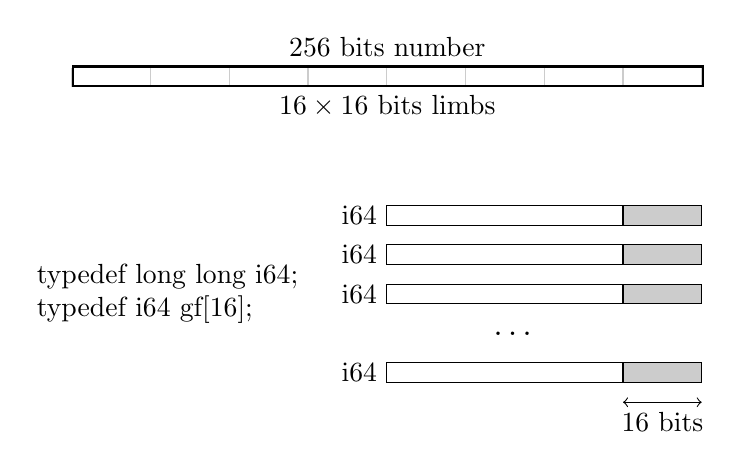
\begin{tikzpicture}[textstyle/.style={black, anchor= south west, align=center}]


			\foreach \x in {0,1,...,8} {
					\draw [black!20] (\x,0) -- (\x,0.25);
				};

			\draw (0,0.25) node[textstyle, minimum width=8cm, minimum height=0.5cm] {$256$ bits number};
			\draw (0,0) node[textstyle, draw=black, thick, minimum width=8cm, minimum height=0.25cm] {};

			\draw (0,-0.5) node[textstyle, minimum width=8cm] {$16 \times 16$ bits limbs};

			\def\yshift{-1.5}
			\def\xshift{4}

			\foreach \y in {0,-0.5,-1,-2} {
					\draw (\xshift+0,\yshift+\y) -- (\xshift+4,\yshift+\y) -- (\xshift+4,\yshift-0.25+\y) -- (\xshift+0,\yshift-0.25+\y) -- cycle;
					\draw [fill=black!20] (\xshift+3,\yshift+\y) -- (\xshift+4,\yshift+\y) -- (\xshift+4,\yshift-0.25+\y) -- (\xshift+3,\yshift-0.25+\y) -- cycle;
					\draw (\xshift,\yshift-0.125+\y) node[anchor= east, align=center] {\TNaCle{i64}};
				}
			\draw (\xshift+2,\yshift-0.125-1.5) node[anchor= east, align=center] {\texttt{...}};

			\draw (3,\yshift-1.125) node[anchor= east, align=left] {\TNaCle{typedef long long i64;}\\
				\TNaCle{typedef i64 gf[16];}};

			\def\yshift{-4}
			\draw [<->] (\xshift+3,\yshift) -- (\xshift+4,\yshift);
			\draw (\xshift+3.5,\yshift) node[textstyle, anchor=north] {$16$ bits};
		\end{tikzpicture}
	\end{center}
\end{frame}


%%%%%%%%%%%%%%%%%%%%%%%%%%%%%%%%%
%
%     SLIDE 5
%
%%%%%%%%%%%%%%%%%%%%%%%%%%%%%%%%%
\begin{frame}[fragile]{Basic Operations}
	\begin{center}

		\begin{lstlisting}[language=Ctweetnacl]
#define FOR(i,n) for (i = 0;i < n;++i)
#define sv static void
typedef long long i64;
typedef i64 gf[16];


sv A(gf o,const gf a,const gf b)    # Addition
{
  int i;
  FOR(i,16) o[i]=a[i]+b[i];         # carrying is done separately
}


sv Z(gf o,const gf a,const gf b)    # Zubtraction
{
  int i;
  FOR(i,16) o[i]=a[i]-b[i];         # carrying is done separately
}


sv M(gf o,const gf a,const gf b)    # Multiplication (school book)
{
  i64 i,j,t[31];
  FOR(i,31) t[i]=0;
  FOR(i,16) FOR(j,16) t[i+j] = a[i]*b[j];
  FOR(i,15) t[i]+=38*t[i+16];
  FOR(i,16) o[i]=t[i];
  car25519(o);                      # carrying
  car25519(o);                      # carrying
}
\end{lstlisting}

	\end{center}
\end{frame}


\section{Formalizing X25519 from RFC 7748}

%%%%%%%%%%%%%%%%%%%%%%%%%%%%%%%%%
%
%     SLIDE 6
%
%%%%%%%%%%%%%%%%%%%%%%%%%%%%%%%%%
\begin{frame}[fragile]{RFC 7748 in Coq}
	\begin{informaltheorem}
		The specification of X25519 in RFC~7748 is formalized by \Coqe{RFC} in Coq.
	\end{informaltheorem}

	More formally:
	\begin{center}
		\begin{lstlisting}[language=Coq]
  Definition RFC (n: list Z) (p: list Z) : list Z :=
    let k := decodeScalar25519 n in
    let u := decodeUCoordinate p in
    let t := montgomery_rec
      255  (* iterate 255 times *)
      k    (* clamped n         *)
      1    (* x_2                *)
      u    (* x_3                *)
      0    (* z_2                *)
      1    (* z_3                *)
      0    (* dummy             *)
      0    (* dummy             *)
      u    (* x_1                *) in
    let a := get_a t in
    let c := get_c t in
    let o := ZPack25519 (Z.mul a (ZInv25519 c))
    in encodeUCoordinate o.
  \end{lstlisting}
	\end{center}
\end{frame}


%%%%%%%%%%%%%%%%%%%%%%%%%%%%%%%%%
%
%     SLIDE 7
%
%%%%%%%%%%%%%%%%%%%%%%%%%%%%%%%%%
\begin{frame}[fragile]{RFC 7748 in Coq}
	\begin{center}
		\begin{lstlisting}[language=Coq]
  Fixpoint montgomery_rec (m : nat) (z : T')
  (a: T) (b: T) (c: T) (d: T) (e: T) (f: T) (x: T) :
  (* a: x2   b: x3   c: z2   d: z3   x: x1  *)
  (T * T * T * T * T * T) :=
  match m with
  | 0%nat => (a,b,c,d,e,f)
  | S n =>
    let r := Getbit (Z.of_nat n) z in                 (* k_t = (k >> t) & 1               *)
      (* swap <- k_t *)
    let (a, b) := (Sel25519 r a b, Sel25519 r b a) in (* (x_2, x_3) = cswap(swap, x_2, x_3)   *)
    let (c, d) := (Sel25519 r c d, Sel25519 r d c) in (* (z_2, z_3) = cswap(swap, z_2, z_3)   *)
    let e := a + c in                                  (* A = x_2 + z_2                     *)
    let a := a - c in                                  (* B = x_2 - z_2                     *)
    let c := b + d in                                  (* C = x_3 + z_3                     *)
    let b := b - d in                                  (* D = x_3 - z_3                     *)
    let d := e ^2 in                                    (* AA = A^2                         *)
    let f := a ^2 in                                    (* BB = B^2                         *)
    let a := c * a in                                  (* CB = C * B                      *)
    let c := b * e in                                  (* DA = D * A                      *)
    let e := a + c in                                  (* x_3 = (DA + CB)^2                 *)
    let a := a - c in                                  (* z_3 = x_1 * (DA - CB)^2            *)
    let b := a ^2 in                                    (* z_3 = x_1 * (DA - CB)^2            *)
    let c := d - f in                                  (* E = AA - BB                     *)
    let a := c * C_121665 in                           (* z_2 = E * (AA + a24 * E)         *)
    let a := a + d in                                  (* z_2 = E * (AA + a24 * E)         *)
    let c := c * a in                                  (* z_2 = E * (AA + a24 * E)         *)
    let a := d * f in                                  (* x_2 = AA * BB                    *)
    let d := b * x in                                  (* z_3 = x_1 * (DA - CB)^2            *)
    let b := e ^2 in                                    (* x_3 = (DA + CB)^2                 *)
    let (a, b) := (Sel25519 r a b, Sel25519 r b a) in (* (x_2, x_3) = cswap(swap, x_2, x_3)   *)
    let (c, d) := (Sel25519 r c d, Sel25519 r d c) in (* (z_2, z_3) = cswap(swap, z_2, z_3)   *)
    montgomery_rec n z a b c d e f x
  end.
  \end{lstlisting}
	\end{center}
\end{frame}


%%%%%%%%%%%%%%%%%%%%%%%%%%%%%%%%%
%
%     SLIDE 8
%
%%%%%%%%%%%%%%%%%%%%%%%%%%%%%%%%%
\begin{frame}[fragile]{RFC 7748 in Coq}
	\begin{informaltheorem}
		Let \Coqe{ZofList} : $\Z \rightarrow \texttt{list}~\Z \rightarrow \Z$,
		a function given $n$ and a list $l$ returns its little endian decoding with radix $2^n$.
	\end{informaltheorem}
	\begin{lstlisting}[language=Coq]
  Fixpoint ZofList {n:Z} (a:list Z) : Z :=
    match a with
    | [] => 0
    | h :: q => h + 2^n * ZofList q
    end.
  \end{lstlisting}

	\begin{informaltheorem}
		Let \Coqe{ListofZ32} : $\Z \rightarrow \Z \rightarrow \texttt{list}~\Z$, given
		$n$ and $a$ returns $a$'s little-endian encoding as a list with radix $2^n$.
	\end{informaltheorem}
	\begin{lstlisting}[language=Coq]
  Fixpoint ListofZn_fp {n:Z} (a:Z) (f:nat) : list Z :=
  match f with
    | 0%nat => []
    | S fuel => (a mod 2^n) :: ListofZn_fp (a/2^n) fuel
  end.

  Definition ListofZ32 {n:Z} (a:Z) : list Z :=
    ListofZn_fp n a 32.
  \end{lstlisting}
\end{frame}


%%%%%%%%%%%%%%%%%%%%%%%%%%%%%%%%%
%
%     SLIDE 9
%
%%%%%%%%%%%%%%%%%%%%%%%%%%%%%%%%%
\begin{frame}[fragile]{RFC 7748 in Coq}

	\Coqe{ListofZ32} and \Coqe{ZofList} are inverse to each other.
	\begin{lstlisting}[language=Coq]
  Lemma ListofZ32_ZofList_Zlength: forall (l:list Z),
    Forall (fun x => 0 <= x < 2^n) l ->
    Zlength l = 32 ->
    ListofZ32 n (ZofList n l) = l.
  Qed.
  \end{lstlisting}

	~\\

	With those tools at hand, we formally define the decoding and
	encoding as specified in the RFC.

	\begin{lstlisting}[language=Coq]
  Definition decodeScalar25519 (l: list Z) : Z :=
    ZofList 8 (clamp l).

  Definition decodeUCoordinate (l: list Z) : Z :=
    ZofList 8 (upd_nth 31 l
      (Z.land (nth 31 l 0) 127)).

  Definition encodeUCoordinate (x: Z) : list Z :=
    ListofZ32 8 x.
  \end{lstlisting}

\end{frame}


\section{From C to Coq}

%%%%%%%%%%%%%%%%%%%%%%%%%%%%%%%%%
%
%     SLIDE 10
%
%%%%%%%%%%%%%%%%%%%%%%%%%%%%%%%%%
\begin{frame}[fragile]{Hoare logic 101}
	\centering
	$$\{{\color{doc@lstnumbers}\textbf{Pre}}\}\texttt{~Prog~}\{{\color{doc@lstdirective}\textbf{Post}}\}$$
	where ${\color{doc@lstnumbers}\textbf{Pre}}$ and ${\color{doc@lstdirective}\textbf{Post}}$
	are assertions and \texttt{Prog} is a fragment of code.

	``when the precondition  ${\color{doc@lstnumbers}\textbf{Pre}}$ is met,
	executing \texttt{Prog} will yield postcondition ${\color{doc@lstdirective}\textbf{Post}}$''.

	~\\

	Sequent Rule in Hoare logic:
	\begin{prooftree}
		\AxiomC{$\{P\}C_1\{Q\}$}
		\AxiomC{$\{Q\}C_2\{R\}$}
		\LeftLabel{Hoare-Seq}
		\BinaryInfC{$\{P\}C_1;C_2\{R\}$}
	\end{prooftree}
\end{frame}


%%%%%%%%%%%%%%%%%%%%%%%%%%%%%%%%%
%
%     SLIDE 11
%
%%%%%%%%%%%%%%%%%%%%%%%%%%%%%%%%%
\begin{frame}[fragile]{Proving with VST}
	\begin{center}

		\begin{tikzpicture}[textstyle/.style={black, anchor= south west, align=center}]
			\draw (2.75,0) node[textstyle, anchor=west, draw=none, fill=doc@lstbackground, thick, minimum width=5.5cm,minimum height=5cm] {};
			\node[inner sep=0pt] (russell) at (5.5,1.5) {
\includegraphics[width=.1\textwidth]{coq_logo.png}};
			\node[inner sep=0pt] (russell) at (5.5,-1.5) {
\includegraphics[width=.15\textwidth]{chain.png}};
			\draw (-1,0) node[textstyle, anchor=east, draw=black, thick, minimum width=1cm,minimum height=2cm] {code.c};
			\draw (0.75,-0.5) node[textstyle, anchor=south] {\texttt{clightgen code.c}};
			\draw (4,0) node[textstyle, anchor=east, draw=black, thick, minimum width=1cm,minimum height=2cm] {code.v};
			\draw (8,0) node[textstyle, anchor=east, draw=black, thick, minimum width=1cm,minimum height=2cm] {proofs.v};
			\node[anchor=west,single arrow,draw=red!80!black,fill=red!80!black,minimum width=0.5cm,minimum height=3.25cm] at (-0.75,0) {};
			\node[anchor=west,double arrow,draw=green!60!black,fill=green!60!black,minimum width=0.5cm,minimum height=2.25cm] at (4.25,0) {};
			% \node[anchor=west,double arrow,draw=green!60!black,fill=green!60!black,minimum width=0.5cm,minimum height=2cm] at (3,0) {};
		\end{tikzpicture}

	\end{center}
\end{frame}


%%%%%%%%%%%%%%%%%%%%%%%%%%%%%%%%%
%
%     SLIDE 12
%
%%%%%%%%%%%%%%%%%%%%%%%%%%%%%%%%%
\begin{frame}[fragile]{Specification: Addition}
	\begin{center}
		\begin{lstlisting}[language=Coq]
Fixpoint Low.A (a b : list \Z) : list \Z :=
  match a,b with
  | [], q => q
  | q,[] => q
  | h1::q1,h2::q2 => (Z.add h1 h2) :: Low.A q1 q2
  end.
Notation "a \boxplus b" := (Low.A a b) (at level 60).


Corollary A_correct:
  forall (a b: list \Z),
    ZofList 16 (a \boxplus b) = (ZofList 16 a) + (ZofList 16 b).
Qed.


Lemma A_bound_len:
  forall (m1 n1 m2 n2: \Z) (a b: list \Z),
    length a = length b ->
    Forall (fun x => m1 << x << n1) a ->
    Forall (fun x => m2 << x << n2) b ->
      Forall (fun x => m1 + m2 < x < n1 + n2) (a \boxplus b).
Qed.

Lemma A_length_16:
  forall (a b: list \Z),
  length a = 16 ->
  length b = 16 ->
    length (a \boxplus b) = 16.
Qed.
\end{lstlisting}

	\end{center}
\end{frame}


%%%%%%%%%%%%%%%%%%%%%%%%%%%%%%%%%
%
%     SLIDE 13
%
%%%%%%%%%%%%%%%%%%%%%%%%%%%%%%%%%
\begin{frame}[fragile]{Verification: Addition (with VST)}
	\begin{center}
		\begin{tikzpicture}
			\draw (0,0) node[below left] {
				\begin{lstlisting}[language=CoqVST]
Definition A_spec :=
DECLARE _A
WITH
  v_o: val, v_a: val, v_b: val,
  sh : share,
  o : list val,
  a : list Z, amin : Z, amax : Z,
  b : list Z, bmin : Z, bmax : Z,

(*------------------------------------------*)
PRE [ _o OF (tptr tlg), _a OF (tptr tlg), _b OF (tptr tlg) ]
    PROP  (writable_share sh;
          (* For soundness *)                         (* For bounds propagation *)
           Forall (fun x => -2^62 < x < 2^62) a;          Forall (fun x => amin < x < amax) a;
           Forall (fun x => -2^62 < x < 2^62) b;          Forall (fun x => bmin < x < bmax) b;

           Zlength a = 16; Zlength b = 16; Zlength o = 16)
    LOCAL (temp _a v_a; temp _b v_b; temp _o v_o)
    SEP   (sh [{ v_o }] <<(lg16)-- o;
           sh [{ v_a }] <<(lg16)-- mVI64 a;
           sh [{ v_b }] <<(lg16)-- mVI64 b)

  (*------------------------------------------*)
  POST [ tvoid ]
      PROP ( (* Bounds propagation *)
            Forall (fun x => amin + bmin < x < amax + bmax) (Low.A a b)
            Zlength (A a b) = 16;
           )
      LOCAL()
      SEP (sh [{ v_o }] <<(lg16)-- mVI64 (Low.A a b);
           sh [{ v_a }] <<(lg16)-- mVI64 a;
           sh [{ v_b }] <<(lg16)-- mVI64 b).
\end{lstlisting}
			};
			\draw (1.5,0) node[below left] {
				\begin{lstlisting}[language=Ctweetnacl]
sv A(gf o,const gf a,const gf b)
{
  int i;
  FOR(i,16) o[i]=a[i]+b[i];
}
\end{lstlisting}
			};
			\draw[black] (1.5,0) -- (1.5,-1.35) -- (-2.35,-1.35) -- (-2.35,0) -- cycle;
		\end{tikzpicture}
	\end{center}
\end{frame}


%%%%%%%%%%%%%%%%%%%%%%%%%%%%%%%%%
%
%     SLIDE 14
%
%%%%%%%%%%%%%%%%%%%%%%%%%%%%%%%%%
\begin{frame}[fragile]{Crypto\_Scalarmult and RFC}

	\begin{enumerate}
		\item We define \coqe{Low.A}; \coqe{Low.M}; \coqe{Low.Sq}; \coqe{Low.Zub}; \coqe{Unpack25519}; \coqe{clamp}; \coqe{Pack25519};
		      \coqe{Inv25519}; \coqe{car25519} to have the same behavior as the low level C code.
		\item We define \coqe{Crypto_Scalarmult} with \coqe{Low.A}; \coqe{Low.M}; \coqe{Low.Sq}; \coqe{Low.Zub}; \coqe{Unpack25519}; \coqe{clamp}; \coqe{Pack25519};
		      \coqe{Inv25519}; \coqe{car25519}; \coqe{montgomery_rec}.
		\item We prove that \coqe{Low.M}; \coqe{Low.A}; \coqe{Low.Sq}; \coqe{Low.Zub};
		      \coqe{Unpack25519}; \coqe{clamp}; \coqe{Pack25519}; \coqe{Inv25519}; \coqe{car25519} have the same behavior over \coqe{list Z}
		      as their equivalent over \coqe{Z} with \coqe{:GF} (in \Zfield).
		\item We prove that \coqe{Crypto_Scalarmult} performs the same computation as \coqe{RFC}.
	\end{enumerate}

	\begin{lstlisting}[language=Coq, basicstyle=\normalsize]
Lemma Crypto_Scalarmult_RFC_eq :
  forall (n: list Z) (p: list Z),
  Zlength n = 32 ->
  Zlength p = 32 ->
  Forall (fun x => 0 <= x /\ x < 2^8) n ->
  Forall (fun x => 0 <= x /\ x < 2^8) p ->
  Crypto_Scalarmult n p = RFC n p.
Qed.
\end{lstlisting}

\end{frame}


%%%%%%%%%%%%%%%%%%%%%%%%%%%%%%%%%
%
%     SLIDE 15
%
%%%%%%%%%%%%%%%%%%%%%%%%%%%%%%%%%
\begin{frame}[fragile]{Hoare Triple of crypto\_scalarmult}
	\begin{lstlisting}[language=CoqVST]
Definition crypto_scalarmult_spec :=
DECLARE _crypto_scalarmult_curve25519_tweet
WITH
  v_q: val, v_n: val, v_p: val, c121665:val,
  sh : share,
  q : list val, n : list Z, p : list Z
(*------------------------------------------*)
PRE [ _q OF (tptr tuchar), _n OF (tptr tuchar), _p OF (tptr tuchar) ]
PROP (writable_share sh;
      Forall (fun x => 0 <= x < 2^8) p;
      Forall (fun x => 0 <= x < 2^8) n;
      Zlength q = 32;
      Zlength n = 32;
      Zlength p = 32)
LOCAL(temp _q v_q; temp _n v_n; temp _p v_p; gvar __121665 c121665)
SEP  (sh [{ v_q }] <<(uch32)-- q;
      sh [{ v_n }] <<(uch32)-- mVI n;
      sh [{ v_p }] <<(uch32)-- mVI p;
      Ews [{ c121665 }] <<(lg16)-- mVI64 c_121665)
(*------------------------------------------*)
POST [ tint ]
PROP (Forall (fun x => 0 <= x < 2^8) (RFC n p);
      Zlength (RFC n p) = 32)
LOCAL(temp ret_temp (Vint Int.zero))
SEP  (sh [{ v_q }] <<(uch32)-- mVI (RFC n p);
      sh [{ v_n }] <<(uch32)-- mVI n;
      sh [{ v_p }] <<(uch32)-- mVI p;
      Ews [{ c121665 }] <<(lg16)-- mVI64 c_121665
\end{lstlisting}
\end{frame}


%%%%%%%%%%%%%%%%%%%%%%%%%%%%%%%%%
%
%     SLIDE 16
%
%%%%%%%%%%%%%%%%%%%%%%%%%%%%%%%%%
\begin{frame}[fragile]{TweetNaCl implements correctly the RFC}
	\begin{informaltheorem}
		The implementation of X25519 in TweetNaCl (\TNaCle{crypto_scalarmult})\\
		matches the specifications of RFC~7748 (\Coqe{RFC}).
	\end{informaltheorem}

	More formally:
	\begin{lstlisting}[language=Coq, basicstyle=\normalsize]
  Theorem body_crypto_scalarmult:
    (* VST boiler plate. *)
    semax_body
      (* Clight translation of TweetNaCl. *)
      Vprog
      (* Hoare triples for fct calls. *)
      Gprog
      (* fct we verify. *)
      f_crypto_scalarmult_curve25519_tweet
      (* Our Hoare triple, see below. *)
      crypto_scalarmult_spec.
  \end{lstlisting}
\end{frame}


\section{Formalization of Elliptic Curves}

%%%%%%%%%%%%%%%%%%%%%%%%%%%%%%%%%
%
%     SLIDE 17
%
%%%%%%%%%%%%%%%%%%%%%%%%%%%%%%%%%
\begin{frame}[fragile]{Formal definition of a point}
	\begin{center}
		\begin{lstlisting}[language=Coq, basicstyle=\normalsize]
Inductive point (\K: Type) : Type :=
  (* A point is either at Infinity  *)
  | EC_Inf : point \K
  (* or (x,y) *)
  | EC_In  : \K -> \K -> point \K.

Notation "\infty" := (@EC_Inf _).
Notation "(| x , y |)" := (@EC_In _ x y).



(* Get the x coordinate of p or 0 *)
Definition point_x0 (p : point \K) :=
  if p is (|x, _ |) then x else 0.

Notation "p.x" := (point_x0 p).
\end{lstlisting}
	\end{center}
	\chapternote{A Formal Library for Elliptic Curves in the Coq Proof Assistant --
		Evmorfia-Iro Bartzia, Pierre-Yves Strub
		\url{https://hal.inria.fr/hal-01102288}}
\end{frame}


%%%%%%%%%%%%%%%%%%%%%%%%%%%%%%%%%
%
%     SLIDE 18
%
%%%%%%%%%%%%%%%%%%%%%%%%%%%%%%%%%
\begin{frame}[fragile]{Formal definition of a curve}

	\begin{dfn}
		Let $a \in \K \backslash \{-2, 2\}$, and $b \in \K \backslash \{ 0\}$. The \textit{elliptic curve} $M_{a,b}$ is defined by the equation:
		$$by^2 = x^3 + ax^2 + x,$$
		$M_{a,b}(\K)$ is the set of all points $(x,y) \in \K^2$ satisfying the $M_{a,b}$ along with an additional formal\\
		point $\Oinf$, ``at infinity''.
	\end{dfn}

	\begin{center}
		\begin{lstlisting}[language=Coq, basicstyle=\normalsize]
(* B y = x^3 + A x^2 + x *)
Record mcuType := { A: \K; B: \K; _ : B != 0; _ : A^2 != 4 }

(* is a point p on the curve? *)
Definition oncurve (p : point K) :=
if p is (| x, y |)
  then cB * y^+2 == x^+3 + cA * x^+2 + x
  else true.

(* We define a point on a curve as a point and the proof that it is on the curve *)
Inductive mc : Type := MC p of oncurve p.
\end{lstlisting}
	\end{center}
\end{frame}


%%%%%%%%%%%%%%%%%%%%%%%%%%%%%%%%%
%
%     SLIDE 19
%
%%%%%%%%%%%%%%%%%%%%%%%%%%%%%%%%%
\begin{frame}[fragile]{Formal definition of the operations over a curve}
	\begin{center}
		\begin{lstlisting}[language=Coq, basicstyle=\normalsize]
Definition neg (p: point \K) :=
  if p is (| x, y |) then (| x, - y |) else \infty.


Definition add (p1 p2: point \K) :=
    match p1 , p2 with
    | \infty, _ => p2                                 (* If one point is infinity *)
    | _, \infty => p1                                 (* If one point is infinity *)

    | (| x1, y1 |), (| x2, y2 |) =>
      if x1 == x2 then
        if (y1 == y2) && (y1 != 0) then ...                         (* If p1 = p2 *)
        else
          \infty
      else                                                      (* If p1 <> p2 *)
        let s := (y2 - y1) / (x2 - x1) in
        let xs := s^2 * B - A - x1 - x2 in
         (| xs, -s * (xs - x1) - y1|)
    end


Notation "- x" := (neg x).
Notation "x + y" := (add x y).
Notation "x - y" := (x + (- y)).
\end{lstlisting}
	\end{center}
\end{frame}


%%%%%%%%%%%%%%%%%%%%%%%%%%%%%%%%%
%
%     SLIDE 20
%
%%%%%%%%%%%%%%%%%%%%%%%%%%%%%%%%%
\begin{frame}[fragile]{Projections}
	% \begin{center}
	We define $\chi$ and $\chi_0$ to return the \xcoord of points on a curve.
	\begin{dfn}Let $\chi$ and $\chi_0$:\\
		-- $\chi : M_{a,b}(\K) \to \K \cup \{\infty\}$\\
		such that $\chi(\Oinf) = \infty$ and $\chi((x,y)) = x$.\\
		-- $\chi_0 : M_{a,b}(\K) \to \K$\\
		such that $\chi_0(\Oinf) = 0$ and $\chi_0((x,y)) = x$.
	\end{dfn}

	~\\

	Montgomery curves make use of projective coordinates. Points are represented with triples $(X:Y:Z)$,\\
	with the exception of $(0:0:0)$

	For all $\lambda \neq 0$, the triples $(X:Y:Z)$ and $(\lambda X:\lambda Y:\lambda Z)$ represent the same point.\\
	For $Z\neq 0$, the projective point $(X:Y:Z)$ corresponds to the point $(X/Z,Y/Z)$ on the affine plane.\\
	Likewise the point $(X,Y)$ on the affine plane corresponds to $(X:Y:1)$ on the projective plane.

\end{frame}


%%%%%%%%%%%%%%%%%%%%%%%%%%%%%%%%%
%
%     SLIDE 21
%
%%%%%%%%%%%%%%%%%%%%%%%%%%%%%%%%%
\begin{frame}{xADD}
	\begin{lemma}
		Let $M_{a,b}$ be a Montgomery curve such that $a^2-4$ is not a square in \K, and
		let $X_1, Z_1, X_2, Z_2, X_4, Z_4 \in \K$, such that $(X_1,Z_1) \neq (0,0)$,
		$(X_2,Z_2) \neq (0,0)$, $X_4 \neq 0$ and $Z_4 \neq 0$.
		Define
		\begin{align*}
			X_3 & = Z_4((X_1 - Z_1)(X_2+Z_2) + (X_1+Z_1)(X_2-Z_2))^2  \\
			Z_3 & = X_4((X_1 - Z_1)(X_2+Z_2) - (X_1+Z_1)(X_2-Z_2))^2,
		\end{align*}
		then for any point $P_1$ and $P_2$ in $M_{a,b}(\K)$ such that
		$X_1/Z_1 = \chi(P_1), X_2/Z_2 = \chi(P_2)$, and $X_4/Z_4 = \chi(P_1 - P_2)$,
		we have $X_3/Z_3 = \chi(P_1+P_2)$.\\
		\textbf{Remark:}
		These definitions should be understood in $\K \cup \{\infty\}$.
		If $x\ne 0$ then we define $x/0 = \infty$.
	\end{lemma}
\end{frame}


%%%%%%%%%%%%%%%%%%%%%%%%%%%%%%%%%
%
%     SLIDE 22
%
%%%%%%%%%%%%%%%%%%%%%%%%%%%%%%%%%
\begin{frame}{xDBL}
	\begin{lemma}
		Let $M_{a,b}$ be a Montgomery curve such that $a^2-4$ is not a square in \K, and
		let $X_1, Z_1 \in \K$, such that $(X_1,Z_1) \neq (0,0)$. Define
		\begin{align*}
			c   & = (X_1 + Z_1)^2 - (X_1 - Z_1)^2                   \\
			X_3 & = (X_1 + Z_1)^2(X_1-Z_1)^2                        \\
			Z_3 & = c\Big((X_1 + Z_1)^2+\frac{a-2}{4}\times c\Big),
		\end{align*}
		then for any point $P_1$ in $M_{a,b}(\K)$ such that $X_1/Z_1 = \chi(P_1)$,
		we have $X_3/Z_3 = \chi(2P_1)$.
	\end{lemma}
\end{frame}


%%%%%%%%%%%%%%%%%%%%%%%%%%%%%%%%%
%
%     SLIDE 23
%
%%%%%%%%%%%%%%%%%%%%%%%%%%%%%%%%%
\begin{frame}[fragile]{Correctness of the Montgomery ladder}

	By combinning the Montgomery ladder with the previous formula, we define a ladder \coqe{opt_montgomery} (in which $\K$ has not been fixed yet).

	\begin{hypothesis}
		$a^2-4$ is not a square in \K.
	\end{hypothesis}

	We prove its correctness.
	\begin{theorem}
		\label{thm:montgomery-ladder-correct}
		For all $n, m \in \N$, $x \in \K$, $P \in M_{a,b}(\K)$,
		if $\chi_0(P) = x$ then \coqe{opt_montgomery} returns $\chi_0(n \cdot P)$
	\end{theorem}
	\begin{lstlisting}[language=Coq, basicstyle=\normalsize]
Theorem opt_montgomery_ok (n m: nat) (x : K) :
  n < 2^m ->
  forall (p : mc M), p#x0 = x
  (* if x is the \xcoord of P *)
  -> opt_montgomery n m x = (p *+ n)#x0.
  (* opt_montgomery n m xp is the \xcoord of n \cdot P *).
Qed.
  \end{lstlisting}

\end{frame}


%%%%%%%%%%%%%%%%%%%%%%%%%%%%%%%%%
%
%     SLIDE 24
%
%%%%%%%%%%%%%%%%%%%%%%%%%%%%%%%%%
\begin{frame}[standout]
	\begin{center}
		{  \huge
			Problem !\\~\\
			$a^2-4$ is a square in $\F{p^2}$}
	\end{center}
\end{frame}


%%%%%%%%%%%%%%%%%%%%%%%%%%%%%%%%%
%
%     SLIDE 25
%
%%%%%%%%%%%%%%%%%%%%%%%%%%%%%%%%%
\begin{frame}[fragile]{Curve25519 ladder}
	% \begin{center}
	\begin{lstlisting}[language=Coq, basicstyle=\normalsize]
(* a^2-4 is not a square in \GF. *)
Fact a_not_square : forall x: Zmodp.type,
  x^+2 != (Zmodp.pi 486662)^+2 - 4%:R.

(* 2 is not a square in \GF. *)
Fact two_not_square : forall x: Zmodp.type,
  x^+2 != 2%:R.
\end{lstlisting}

	We now consider $M_{486662,1}(\F{p})$ and $M_{486662,2}(\F{p})$, one of its quadratic twists.

	\begin{dfn}
		%Let the following instantiations of \aref{alg:montgomery-ladder}:\\
		We instantiate \coqe{opt_montgomery} in two specific ways:\\
		-- $Curve25519\_Fp(n,x)$ for $M_{486662,1}(\F{p})$.\\
		-- $Twist25519\_Fp(n,x)$ for $M_{486662,2}(\F{p})$.
	\end{dfn}

	$Curve25519\_Fp(n,x)$ and $Twist25519\_Fp(n,x)$ do not depend on $b$.
	\begin{lstlisting}[language=Coq, basicstyle=\normalsize]
Lemma curve_twist_eq: forall n x,
  curve25519_Fp_ladder n x = twist25519_Fp_ladder n x.
Qed.
\end{lstlisting}
\end{frame}


%%%%%%%%%%%%%%%%%%%%%%%%%%%%%%%%%
%
%     SLIDE 26
%
%%%%%%%%%%%%%%%%%%%%%%%%%%%%%%%%%
\begin{frame}[fragile]{Correct on \F{p}}
	We derive the following two lemmas:
	\begin{lemma}
		For all $x \in \F{p},\ n \in \N,\ P \in \F{p} \times \F{p}$,
		such that $P \in M_{486662,1}(\F{p})$ and $\chi_0(P) = x$.\\
		Given $n$ and $x$, $Curve25519\_Fp(n,x) = \chi_0(n \cdot P)$.
	\end{lemma}
	~\\

	\begin{lemma}
		For all $x \in \F{p},\ n \in \N,\ P \in \F{p} \times \F{p}$
		such that $P \in M_{486662,2}(\F{p})$ and $\chi_0(P) = x$.\\
		Given $n$ and $x$, $Twist25519\_Fp(n,x) = \chi_0(n \cdot P)$.
	\end{lemma}
\end{frame}


%%%%%%%%%%%%%%%%%%%%%%%%%%%%%%%%%
%
%     SLIDE 27
%
%%%%%%%%%%%%%%%%%%%%%%%%%%%%%%%%%
\begin{frame}[fragile]{On the Twist or the Curve over \F{p}}
	As 2 is not a square in \F{p} we have:
	\begin{lemma}
		For all $x$ in $\F{p}$, there exists $y$ in $\F{p}$ such that
		$y^2 = x\ \lor\ 2y^2 = x$
	\end{lemma}

	Thus:
	\begin{lemma}
		For all $x \in \F{p}$, there exists a point $P$ in $M_{486662,1}(\F{p})$ or
		in $M_{486662,2}(\F{p})$ such that the \xcoord of $P$ is $x$.
	\end{lemma}

	And formally:
	\begin{lstlisting}[language=Coq, basicstyle=\normalsize]
Lemma x_is_on_curve_or_twist:
  forall x : Zmodp.type,
  (exists (p : mc curve25519_mcuType), p#x0 = x) \/
  (exists (p' : mc twist25519_mcuType), p'#x0 = x).
Qed.
\end{lstlisting}
\end{frame}


%%%%%%%%%%%%%%%%%%%%%%%%%%%%%%%%%
%
%     SLIDE 28
%
%%%%%%%%%%%%%%%%%%%%%%%%%%%%%%%%%
\begin{frame}{From \F{p} to \F{p^2} and vice-versa}
	We define the two morphism:
	\begin{dfn}
		Define the functions $\varphi_c$, $\varphi_t$ and $\psi$\\
		-- $\varphi_c: M_{486662,1}(\F{p}) \mapsto M_{486662,1}(\F{p^2})$ such that $\varphi((x,y)) = ((x,0), (y,0))$.\\
		-- $\varphi_t: M_{486662,2}(\F{p}) \mapsto M_{486662,1}(\F{p^2})$ such that $\varphi((x,y)) = ((x,0), (0,y))$.\\
		-- $\psi: \F{p^2} \mapsto \F{p}$ such that $\psi(x,y) = (x)$.
	\end{dfn}

	And prove:
	\begin{lemma}
		For all $n \in \N$, for all point $P\in\F{p}\times\F{p}$ on the curve
		$M_{486662,1}(\F{p})$ (respectively on the quadratic twist $M_{486662,2}(\F{p})$), we have:
		\begin{align*}
			P \in M_{486662,1}(\F{p}) & \implies \varphi_c(n \cdot P) = n \cdot \varphi_c(P) \\
			P \in M_{486662,2}(\F{p}) & \implies \varphi_t(n \cdot P) = n \cdot \varphi_t(P)
		\end{align*}
	\end{lemma}

	Notice that:
	\begin{align*}
		\forall P \in M_{486662,1}(\F{p}),\ \ \psi(\chi_0(\varphi_c(P))) = \chi_0(P) \\
		\forall P \in M_{486662,2}(\F{p}),\ \ \psi(\chi_0(\varphi_t(P))) = \chi_0(P)
	\end{align*}

\end{frame}


%%%%%%%%%%%%%%%%%%%%%%%%%%%%%%%%%
%
%     SLIDE 29
%
%%%%%%%%%%%%%%%%%%%%%%%%%%%%%%%%%
\begin{frame}[fragile]{with \F{p}-restricted coordinates over \F{p^2}}
	\begin{theorem}
		\label{thm:general-scalarmult}
		For all $n \in \N$, such that $n < 2^{255}$,
		for all $x \in \F{p}$ and $P \in M_{486662,1}(\F{p^2})$ such that $\chi_0(P) = x$,
		$Curve25519\_Fp(n,x)$ computes $\chi_0(n \cdot P)$.
	\end{theorem}
	which is formalized in Coq as:
	\begin{lstlisting}[language=Coq, basicstyle=\normalsize]
Theorem curve25519_Fp2_ladder_ok:
  forall (n : nat) (x:Zmodp.type),
  (n < 2^255)%nat ->
  forall (p  : mc curve25519_Fp2_mcuType),
  p #x0 = Zmodp2.Zmodp2 x 0 ->
  curve25519_Fp_ladder n x = (p *+ n)#x0 /p.
Qed.
\end{lstlisting}

\end{frame}


%%%%%%%%%%%%%%%%%%%%%%%%%%%%%%%%%
%
%     SLIDE 36
%
%%%%%%%%%%%%%%%%%%%%%%%%%%%%%%%%%
\begin{frame}[fragile]{RFC is correct}
	\begin{informaltheorem}
		The implementation of X25519 in TweetNaCl computes the
		$\F{p}$-restricted \xcoord scalar multiplication on $E(\F{p^2})$ where $p$ is $\p$
		and $E$ is the elliptic curve $y^2 = x^3 + 486662 x^2 + x$.
	\end{informaltheorem}

	\begin{lstlisting}[language=Coq, basicstyle=\normalsize]


  Theorem RFC_Correct: forall (n p : list Z)
    (P:mc curve25519_Fp2_mcuType),
    Zlength n = 32 ->
    Zlength p = 32 ->
    Forall (fun x => 0 <= x /\ x < 2 ^ 8) n ->
    Forall (fun x => 0 <= x /\ x < 2 ^ 8) p ->
    Fp2_x (decodeUCoordinate p) = P#x0 ->
    RFC n p =
      encodeUCoordinate
        ((P *+ (Z.to_nat (decodeScalar25519 n))) _x0).
  Qed.
  \end{lstlisting}
\end{frame}

%%%%%%%%%%%%%%%%%%%%%%%%%%%%%%%%%
%
%     SLIDE 14
%
%%%%%%%%%%%%%%%%%%%%%%%%%%%%%%%%%
\begin{frame}[standout]
	\Huge Thank you.
\end{frame}


\appendix

\section{Equivalences}

%%%%%%%%%%%%%%%%%%%%%%%%%%%%%%%%%
%
%     SLIDE 30
%
%%%%%%%%%%%%%%%%%%%%%%%%%%%%%%%%%
\begin{frame}[fragile]{Generic Operations}
	\begin{center}

		\begin{lstlisting}[language=Coq]
Class Ops (T T': Type) (Mod: T -> T):=
{
  A:   T -> T -> T;                 (* Addition       over T *)
  M:   T -> T -> T;                 (* Multiplication over T *)
  Zub: T -> T -> T;                 (* Subtraction   over T *)
  Sq:  T -> T;                       (* Squaring       over T *)
  C_0: T;                             (* Constant 0       in T *)
  C_1: T;                             (* Constant 1       in T *)
  C_121665: T;                        (* Constant 121665  in T *)
  Sel25519: \Z -> T -> T -> T;      (* Select the 2^nd or 3^rd argument depending of Z *)
  Getbit:   \Z -> T' -> \Z;           (* Return the i^th bit of T' *)

  (* Mod conservation *)
  Mod_ZSel25519_eq : forall b p q,  Mod (Sel25519 b p q) = Sel25519 b (Mod p) (Mod q);
  Mod_ZA_eq :        forall p q,    Mod (A p q)          = Mod (A (Mod p) (Mod q));
  Mod_ZM_eq :        forall p q,    Mod (M p q)          = Mod (M (Mod p) (Mod q));
  Mod_ZZub_eq :      forall p q,    Mod (Zub p q)        = Mod (Zub (Mod p) (Mod q));
  Mod_ZSq_eq :       forall p,      Mod (Sq p)           = Mod (Sq (Mod p));

  Mod_red :          forall p,      Mod (Mod p)          = (Mod p)
}.
\end{lstlisting}
	\end{center}
\end{frame}


%%%%%%%%%%%%%%%%%%%%%%%%%%%%%%%%%
%
%     SLIDE 31
%
%%%%%%%%%%%%%%%%%%%%%%%%%%%%%%%%%
\begin{frame}[fragile]{Generic Montgomery Ladder}
	\begin{center}
		\begin{lstlisting}[language=Coq]
Context {T : Type}.
Context {T' : Type}.
Context {Mod : T -> T}.
Context {O : Ops T T' Mod}.

Fixpoint montgomery_rec (m : \N) (z : T') (a b c d e f x : T) : (T * T * T * T * T * T) :=
  match m with
  | 0 => (a,b,c,d,e,f)
  | S n =>
      let r := Getbit (\Z.of_nat n) z in
      let (a, b) := (Sel25519 r a b, Sel25519 r b a) in
      let (c, d) := (Sel25519 r c d, Sel25519 r d c) in
      let e := A a c in
      let a := Zub a c in
      let c := A b d in
      let b := Zub b d in
      let d := Sq e in
      let f := Sq a in
      let a := M c a in
      let c := M b e in
      let e := A a c in
      let a := Zub a c in
      let b := Sq a in
      let c := Zub d f in
      let a := M c C_121665 in
      let a := A a d in
      let c := M c a in
      let a := M d f in
      let d := M b x in
      let b := Sq e in
      let (a, b) := (Sel25519 r a b, Sel25519 r b a) in
      let (c, d) := (Sel25519 r c d, Sel25519 r d c) in
      montgomery_rec n z a b c d e f x
    end.
\end{lstlisting}
	\end{center}
\end{frame}


%%%%%%%%%%%%%%%%%%%%%%%%%%%%%%%%%
%
%     SLIDE 32
%
%%%%%%%%%%%%%%%%%%%%%%%%%%%%%%%%%
\begin{frame}[fragile]{Operations Equivalence}
	\begin{center}

		\begin{lstlisting}[language=Coq]
Class Ops_Mod_P {T T' U:Type}
                {Mod:U -> U} {ModT:T -> T}
                `(Ops T T' ModT) `(Ops U U Mod)  :=
{
P:  T  -> U;    (* Projection from T  to U *)
P': T' -> U;    (* Projection from T' to U *)

A_eq:        forall a b, Mod (P (A a b))   = Mod (A (P a) (P b));
M_eq:        forall a b, Mod (P (M a b))   = Mod (M (P a) (P b));
Zub_eq:      forall a b, Mod (P (Zub a b)) = Mod (Zub (P a) (P b));
Sq_eq:       forall a,   Mod (P (Sq a))    = Mod (Sq (P a));

C_121665_eq: P C_121665 = C_121665;
C_0_eq:      P C_0 = C_0;
C_1_eq:      P C_1 = C_1;

Sel25519_eq: forall b p q,  Mod (P (Sel25519 b p q)) = Mod (Sel25519 b (P p) (P q));
Getbit_eq:   forall i p,    Getbit i p = Getbit i (P' p);
}.
\end{lstlisting}
	\end{center}
\end{frame}


%%%%%%%%%%%%%%%%%%%%%%%%%%%%%%%%%
%
%     SLIDE 33
%
%%%%%%%%%%%%%%%%%%%%%%%%%%%%%%%%%
\begin{frame}[fragile]{Generic Montgomery Equivalence}
	\begin{center}

		\begin{lstlisting}[language=Coq]
Context {T:    Type}.
Context {T':   Type}.
Context {U:    Type}.
Context {ModT: T -> T}.
Context {Mod:  U -> U}.
Context {TO:   Ops T T' ModT}.
Context {UO:   Ops U U  Mod}.
Context {UTO: @Ops_Mod_P T T' U Mod ModT TO UO}.


(* montgomery_rec over T is equivalent to montgomery_rec over U *)
Corollary montgomery_rec_eq_a: forall (n:\N) (z:T') (a b c d e f x: T),
  Mod (P (get_a (montgomery_rec n z a b c d e f x))) =                              (* over T *)
  Mod (get_a (montgomery_rec n (P' z) (P a) (P b) (P c) (P d) (P e) (P f) (P x))).  (* over U *)
Qed.

Corollary montgomery_rec_eq_c: forall (n:\N) (z:T') (a b c d e f x: T),
  Mod (P (get_c (montgomery_rec n z a b c d e f x))) =                              (* over T *)
  Mod (get_c (montgomery_rec n (P' z) (P a) (P b) (P c) (P d) (P e) (P f) (P x))).  (* over U *)
Qed.
\end{lstlisting}
	\end{center}
\end{frame}


%%%%%%%%%%%%%%%%%%%%%%%%%%%%%%%%%
%
%     SLIDE 34
%
%%%%%%%%%%%%%%%%%%%%%%%%%%%%%%%%%
\begin{frame}[fragile]{Instanciating}
	% \vspace{-0.5cm}
	\begin{center}
		\begin{lstlisting}[language=Coq]
Definition modP (x: \Z) := x mod 2^255-19.

(* Operations over \Z *)
Instance Z_Ops :      Ops \Z \Z modP := {}.

(* Operations over \GF *)
Instance Z25519_Ops : Ops \GF \N id := {}.

(* Equivalence between \Z (with modP) and \Z *)
Instance Zmod_Z_Eq :   @Ops_Mod_P Z Z Z modP modP Z_Ops Z_Ops :=
{ P := modP; P' := id }.

(* Equivalence between \Z (with modP) and \GF *)
Instance Z25519_Z_Eq : @Ops_Mod_P Zmodp.type nat Z modP id Z25519_Ops Z_Ops :=
{ P := val; P' := \Z.of_nat }.

Inductive List16 (T:Type) := Len (l:list T): Zlength l = 16 -> List16 T.
Inductive List32B :=         L32B (l:list \Z): Forall (fun x => 0 <= x << 2^8) l -> List32B.

(* Operations over List16,List32 *)
Instance List16_Ops : Ops (@List16 \Z) List32B id := {}.

(* Equivalence between List16,List32 and \Z *)
Instance List16_Z_Eq : @Ops_Mod_P (@List16 \Z) (List32B) Z modP id List16_Ops Z_Ops :=
{  P l := (ZofList 16 (List16_to_List l));       P' l := (ZofList 8 (List32_to_List l));  }.

(* Operations over list of \Z *)
Instance List_Z_Ops : Ops (list \Z) (list \Z) id := {}.

(* Equivalence between List16,List32 and list of \Z *)
Instance List16_List_Z_Eq : @Ops_Mod_P (List16 \Z) (List32B) (list \Z) id id List16_Ops List_Z_Ops :=
{  P := List16_to_List;         P' := List32_to_List      }.
\end{lstlisting}
	\end{center}
\end{frame}


%%%%%%%%%%%%%%%%%%%%%%%%%%%%%%%%%
%
%     SLIDE 35
%
%%%%%%%%%%%%%%%%%%%%%%%%%%%%%%%%%
\begin{frame}[fragile]{Full Equivalence}
	\vspace{-0.2cm}
	\begin{center}
		\begin{tikzpicture}

			\draw[draw=none,fill=doc@lstbackground] (-8,0.7) -- (6,0.7) -- (6,-7.5) -- (-8,-7.5) -- cycle;
			\draw (-8,-7.5) node[inner sep=0pt, above right] {
\includegraphics[width=.1\textwidth]{coq_logo.png}};

			\draw (0,0) node[above,draw, minimum width=4cm, minimum height=0.65cm] (GF) {\coqes{Ops \GF \N id}};
			\draw (0,-1.5) node[above,draw, minimum width=4cm, minimum height=0.65cm] (Zmod) {\coqes{Ops \Z(with modP) \Z(with modP) modP}};
			\draw (0,-3) node[above,draw, minimum width=4cm, minimum height=0.65cm] (Z) {\coqes{Ops \Z \Z modP}};
			\draw (0,-4.5) node[above,draw, minimum width=4cm, minimum height=0.65cm] (L16) {\coqes{Ops (@List16 \Z) List32B id}};
			\draw (0,-6) node[above,draw, minimum width=4cm, minimum height=0.65cm] (L) {\coqes{Ops (list \Z) (list \Z) id}};
			\draw (5,-4.5) node[above,minimum width=1cm, minimum height=0.65cm] (RFC) {\coqes{RFC n p}};

			\draw[double,<->,>=stealth] (GF.south) -- (Zmod.north) node[midway, right]{\coqes{Z25519_Z_Eq}};
			\draw[double,<->,>=stealth] (Zmod.south) -- (Z.north) node[midway, right]{\coqes{Zmod_Z_Eq}};
			\draw[double,<->,>=stealth] (Z.south) -- (L16.north) node[midway, right]{\coqes{List16_Z_Eq}};
			\draw[double,<->,>=stealth] (L16.south) -- (L.north) node[midway, right]{\coqes{List16_List_Z_Eq}};

			\draw[<-] (GF.west) --++ (-1.5,0) node[left] {\coqes{curve25519_Fp_ladder n xp}}                     node[midway,above] {\scriptsize defined with};
			\draw[<-] (Z.west)  --++ (-1.5,0) node[left] {\coqes{ZCrypto_Scalarmult (ZofList n) (ZofList p)}}  node[midway,above] {\scriptsize defined with};
			\draw[<-] (L.west)  --++ (-1.5,0) node[left] (CSM) {\coqes{Crypto_Scalarmult n p}}                 node[midway,above] {\scriptsize defined with};
			\draw[<-] (L.east) -- (RFC.west)  node[midway,above] {\scriptsize uses};
			\draw[<-] (Z.east) -- (RFC.west)  node[midway,above] {\scriptsize uses};


			\draw (-6.25,-7.4) node[above right,draw,dashed,minimum width=3.5cm, minimum height=0.45cm] (TNACL) {\scriptsize \texttt{tweetnacl.v} (output of clightgen)};

			\draw[double,<->,>=stealth] (CSM.south) -- (TNACL.north) node[midway, right]{
\includegraphics[width=.07\textwidth]{chain.png}};

		\end{tikzpicture}

	\end{center}
\end{frame}



% \section{car25519}
%
% %%%%%%%%%%%%%%%%%%%%%%%%%%%%%%%%%
% %
% %     SLIDE 15
% %
% %%%%%%%%%%%%%%%%%%%%%%%%%%%%%%%%%
%
% \begin{frame}[fragile]{car25519 - specification}
%   \begin{center}
%
% \begin{lstlisting}[language=Ctweetnacl]
%   FOR(i,15) {
%     o[(i+1)]+=o[i]>>16;   # propagate to the next limb
%     o[i]&=0xffff;         # remove the carry
%   }
% \end{lstlisting}
%
% \begin{lstlisting}[language=Coq]
% (*
%   getCarry n m      is equivalent to    m >> n
%   getResidute n m   is equivalent to    m mod 2^n
% *)
%
% Fixpoint Carrying_n (p:\N) (a:\Z) (l:list \Z) : list \Z := match p,a,l with
% | _,    0,[]     => []
% | _,    a,[]     => [a]
% | 0%\N,  a,h::q => (a + h) :: q
% | S p,  a,h :: q => getResidute n (a + h) :: Carrying_n p (getCarry n (a + h)) q
% end.
%
% Corollary CarrynPreserve:
%   forall (m: \N) (l: list \Z),
%     ZofList 16 l = ZofList 16 Carrying_n m 0 l.
% Qed.
% \end{lstlisting}
%   \end{center}
% \end{frame}
%
%
% %%%%%%%%%%%%%%%%%%%%%%%%%%%%%%%%%
% %
% %     SLIDE 16
% %
% %%%%%%%%%%%%%%%%%%%%%%%%%%%%%%%%%
%
% \begin{frame}[fragile]{car25519 - specification}
%   \begin{center}
%
% \begin{lstlisting}[language=Ctweetnacl]
%   o[0]+=38*(o[15]>>16);
%   o[15]&=0xffff;
% \end{lstlisting}
%
% \begin{lstlisting}[language=Coq]
% Definition backCarry (l:list Z) : (list Z) :=
%   match l with
%   | [] => []
%   | h :: q => let v := nth 15 l 0 in
%               (h + 38 * getCarry 16 v) :: slice 14 q ++ [getResidute 16 v]
%   end.
%
% Lemma backCarry_25519:
%   forall (l:list \Z),
%     (length l <= 16)%\N ->
%       (ZofList 16 l) :\GF  = ((ZofList 16 backCarry l) :\GF).
% Qed.
% \end{lstlisting}
%
%   \end{center}
% \end{frame}
%
%
%
% %%%%%%%%%%%%%%%%%%%%%%%%%%%%%%%%%
% %
% %     SLIDE 17
% %
% %%%%%%%%%%%%%%%%%%%%%%%%%%%%%%%%%
%
% \begin{frame}[fragile]{car25519 - correctness \& bounds}
%   \begin{center}
% \begin{lstlisting}[language=Coq]
% Definition car25519 (l:list \Z) : list \Z := backCarry (Carrying_n 16 15 0 l).
%
% Lemma car25519_correct:
%   forall (l: list \Z),
%     (length l = 16)%\N ->
%       (ZofList 16 l) :\GF  = (ZofList 16 car25519 l) :\GF.
% Qed.
%
% Lemma car25519_bound :
%   forall (i: \N) (l: list \Z),
%     (length l = 16)%\N ->
%     (i <> 0)%\N ->
%       nth i (car25519 l) 0 < 2^16.
% Qed.
% \end{lstlisting}
%   \end{center}
% \end{frame}
%
%
%
% %%%%%%%%%%%%%%%%%%%%%%%%%%%%%%%%%
% %
% %     SLIDE 18
% %
% %%%%%%%%%%%%%%%%%%%%%%%%%%%%%%%%%
%
% \begin{frame}[fragile]{car25519 - bounds}
%   \begin{center}
% \begin{lstlisting}[language=Coq]
% Lemma t2256is38 : (2^256 :\GF) = (38 :\GF).
% Proof. compute. reflexivity. Qed.
%
% Definition Zcar25519 (n: \Z) : \Z  :=  38 * getCarry 256 n +  getResidute 256 n.
%
% Lemma Zcar25519_correct:
%   forall (n: \Z), n :\GF = (Zcar25519 n) :\GF.
% Qed.
%
% Lemma Zcar25519_eq_car25519:
%   forall (l : list \Z),
%   (length l = 16)%\N ->
%     Zcar25519 (ZofList l) = ZofList (car25519 l).
% Qed.
% \end{lstlisting}
%
%   \end{center}
% \end{frame}
%
%
% %%%%%%%%%%%%%%%%%%%%%%%%%%%%%%%%%
% %
% %     SLIDE 19
% %
% %%%%%%%%%%%%%%%%%%%%%%%%%%%%%%%%%
%
% \begin{frame}[fragile]{car25519 - bounds}
%   \begin{center}
% \begin{lstlisting}[language=Coq]
% Lemma ZCarry25519_min:
%   forall (x: \Z),
%     0 < x ->
%       0 < Zcar25519 x.
% Qed.
%
% Lemma ZCarry25519_sup_bounds:
%   forall (x: \Z),
%     x < 2 ^ 302 ->
%     0 < x ->
%       Zcar25519 x < 2 ^ 257.
% Qed.
%
% Lemma Zcarry25519_fixpoint :
%   forall (x: \Z),
%   0 < x < 2 ^ 256 ->
%     Zcar25519 x = x.
% Qed.
%
% Theorem doubleCar:
%   forall (x y: \Z),
%     0 <= x < 2 ^ 302 ->
%     y = Zcar25519 x ->
%       Zcar25519 y < 2 ^ 256.
% Qed.
% \end{lstlisting}
%
%   \end{center}
% \end{frame}

\end{document}
